\chapter{ Pruebas y resultados obtenidos }
Las pruebas se realizaron sobre el simulador de redes elásticas ópticas desarrollado en \cite{davalos2019spectrum} con las topologías USNET y NSFNET, la generación de demandas se realiza de manera aleatoria, pero con variaciones de volumen de tráfico. En la figura \ref{fig:traficos} se pueden ver las curvas de rutas activas, siendo el eje \textit{x} el tiempo y el eje \textit{y} la cantidad de rutas activas, para lograr esto inicialmente la simulación inicia con 700 Erlangs y al llegar la utilización de la red a un valor máximo baja a 100 Erlangs, de esta forma conseguimos que la carga de la red no sea constante y podamos acercarnos a un escenario más real. Para el proceso de desfragmentación se utilizó el algoritmo genético propuesto en \cite{davalos2019spectrum}.

El proceso que seguimos para seleccionar el periodo de tiempo en el que el proceso de desfragmentación se ejecutará se puede ver en la figura \ref{fig:simuladorModelo}, donde las características son las citadas en el capítulo 4 sección 4.1, \textit{PB} es la probabilidad de bloqueo calculada por nuestro modelo entrenado, \(PB_{th}\) es el valor seleccionado como umbral para que el proceso de desfragmentación se dispare y \textit{DF} es el proceso de desfragmentación.  

\begin{figure}[h!]
    \centering
    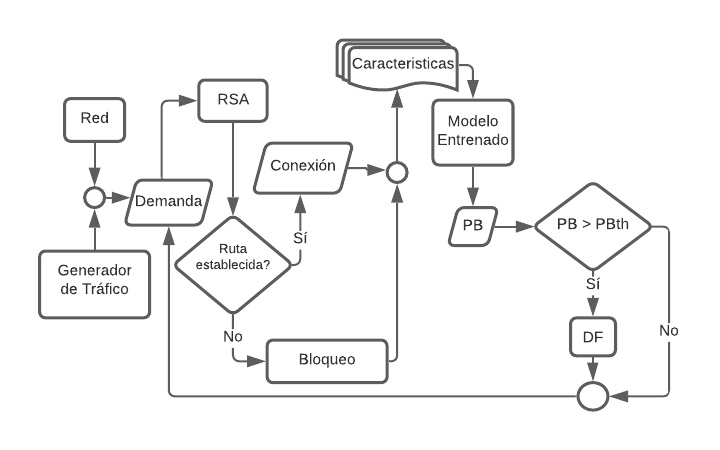
\includegraphics[width=1\textwidth]{capitulos/img/diagramaML6.png}
    \caption{Diagrama simulador / modelo entrenado}
    \label{fig:simuladorModelo}
\end{figure}

Para tener un punto de referencia nuestro modelo se compara con otros dos métodos conocidos:
\begin{itemize}[a)]
    \item Desfragmentación periódica por tiempo fijo: el cual consiste en desfragmentar la red cada cierta cantidad constante de unidades de tiempo.
    \item Desfragmentación por métricas de fragmentación: el cual consiste en desfragmentar cuando la red alcanza cierto valor de alguna métrica, en este caso de BFR.
\end{itemize}

Cada método tiene su propio parámetro encargado de disparar el proceso de desfragmentación y durante las pruebas se hace variar este parámetro hasta tres veces. 

Para elegir este valor tomamos como base la cantidad de desfragmentaciones que realiza el método por tiempo fijo y se buscan valores para los parámetros de los otros métodos de tal manera que ejecuten cantidades similares de desfragmentaciones, así logramos que la comparación se haga de la forma más justa posible.

Las simulaciones se realizaron con los tres métodos bajo las mismas condiciones de variaciones de distribuciones demandas y parámetros, para obtener mayor variación en los resultados este procedimiento se repitió 5 veces.

\section{Objetivos a optimizar}

Para la evaluación de los resultados, considerando dos objetivos globales, medidos al final de cada simulación:

\begin{enumerate}[Obj. 1)]
    \item \textbf{Cantidad de bloqueos(BL):} Suma de las demandas bloqueadas durante la simulación
    \item \textbf{Cantidad de reconfiguraciones(RC):} Número de conexiones reconfiguradas durante los procesos de desfragmentación realizadas durante la simulación. 
\end{enumerate}

Como se trata de dos objetivos a optimizar (BL y RC), buscando minimizar el valor de ambas, para la comparación de los resultados se consideraron dos métricas de desempeño para optimización multi-objetivo \cite{von2014survey}: 

\begin{itemize}
    \item \textbf{Número de soluciones en el Frente Pareto obtenido (SFP):} Para esta primera métrica, se busca determinar el método que contenga el mayor número de soluciones no dominadas que minimicen BL y RC, comparando al mismo tiempo las soluciones de nuestro método propuesto con las soluciones de los otros dos métodos. 
    
     \item \textbf{Cobertura Pareto(CP):} Como segundo método de comparación utilizamos una métrica binaria denominada “Cobertura”, la cual nos permite realizar la comparación de las soluciones óptimas de nuestro método propuesto con los demás métodos tomándolos de a pares.
 
 \begin{equation}
      C(A,B) = \frac{Soluciones\ de\ B\ dominadas\ por\ A}{Soluciones\ totales\ de\ B}  
 \end{equation}
    

\section{Análisis de los resultados}

Se puede observar en la Tabla \ref{tab:frentePareto} que de todas las instancias experimentales que se encuentran en el Frente Pareto, el método propuesto (MP) en este trabajo representa el 52.9\% de los puntos dentro del mismo, lo que indica que este método produce más soluciones no dominadas, indicando una mayor eficiencia en lo que respecta a la minimización de la cantidad de bloqueos y el número de reconfiguraciones en la red.

\begin{table}[h!]
    \centering
    \caption{Tabla de soluciones en el frente pareto}
    \begin{tabular}{|c|c|c|c|c|}
    \hline
    \multirow{2}{*}{\textbf{SIMULACIÓN}} & \multicolumn{4}{c|}{\textbf{Soluciones del Frente Pareto}}\\ \cline{2-5} 
         & \textbf{MP} & \textbf{Tiempo Fijo} & \textbf{BFR} & \textbf{Total}\\
    \hline
    NSFNET & \textbf{9} & 4 & 6 & 19\\
    USNET & \textbf{9} & 4 & 2 & 15\\
    \hline
    
    \end{tabular}
    \label{tab:frentePareto}
\end{table}

 En las figuras \ref{fig:paretoNSFNET} y \ref{fig:paretoUSNET} podemos observar los resultados para los tres diferentes tipos de tráfico, para el caso de la topología USNET (figura \ref{fig:paretoUSNET}), en el frente de soluciones óptimas se aprecia una predominancia del método propuesto en cuanto a cantidad de soluciones. Mientras que en el caso de la topología NSFNET  (figura \ref{fig:paretoNSFNET}), dicha predominancia se puede ver en dos de los tres tipos de tráfico.
 \newpage
 
 \begin{figure}[H]
    \centering
    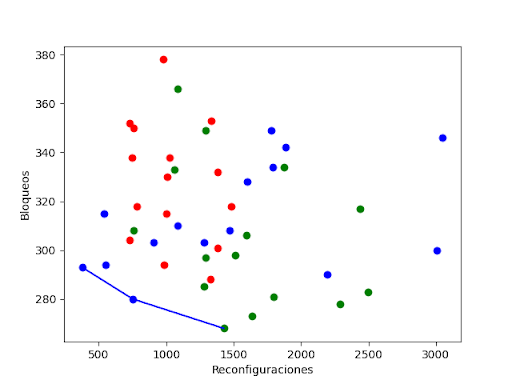
\includegraphics[width=0.9\textwidth]{capitulos/img/nsfnet_pareto_1.png}
    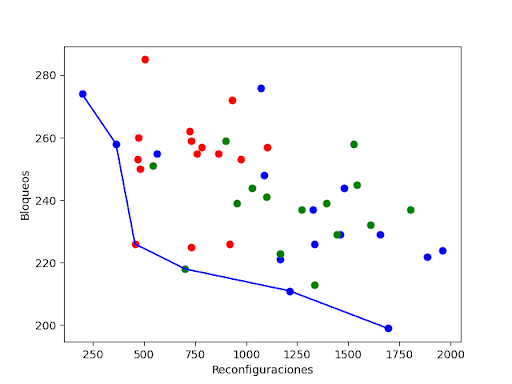
\includegraphics[width=0.9\textwidth]{capitulos/img/nsfnet_pareto_2.png}
    \caption{Gráfico de soluciones en el frente pareto para la topología NSFNET}
 \end{figure}

 \begin{figure}[H]\ContinuedFloat
    \centering
    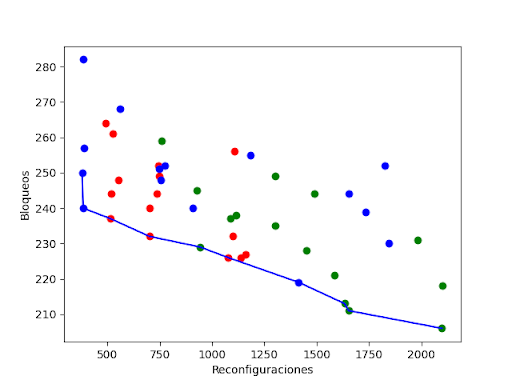
\includegraphics[width=0.9\textwidth]{capitulos/img/nsfnet_pareto_3.png}
    \caption{Gráfico de soluciones en el frente pareto para la topología NSFNET}
    \label{fig:paretoNSFNET}
 \end{figure}

 \begin{figure}[H]
    \centering
    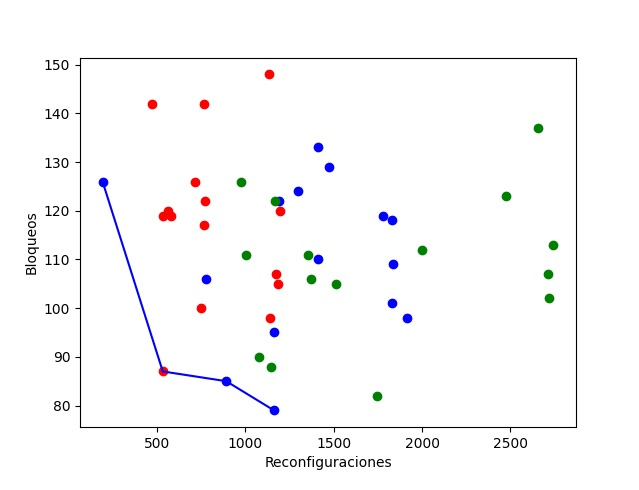
\includegraphics[width=0.9\textwidth]{capitulos/img/paretoUsnetSB.jpg}
    \caption{Gráfico de soluciones en el frente pareto para la topología USNET}
 \end{figure}
\begin{figure}[H] \ContinuedFloat
    \centering
    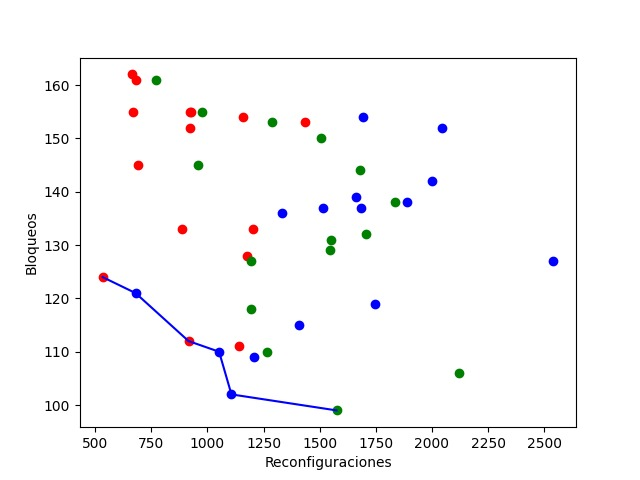
\includegraphics[width=0.9\textwidth]{capitulos/img/paretoUsnetSBSB.jpeg}
    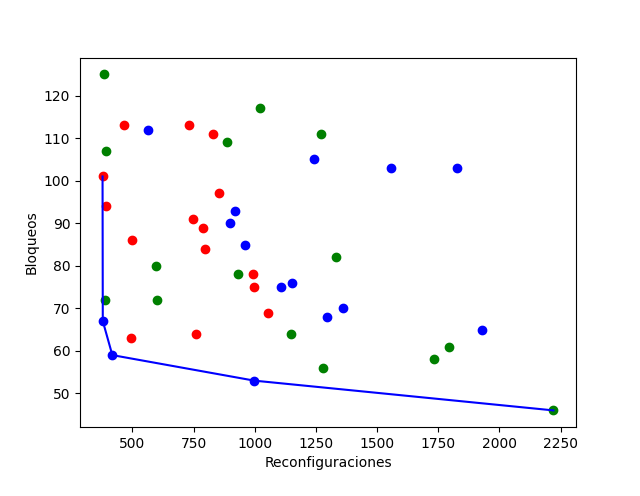
\includegraphics[width=0.9\textwidth]{capitulos/img/paretoUsnetSBS.png}
    \caption{Gráfico de soluciones en el frente pareto para la topología USNET}
    \label{fig:paretoUSNET}
\end{figure}
\newpage

En las tablas \ref{tab:frenteParetoUSNET} y \ref{tab:frenteParetoNSFNET} se presentan los resultados de la métrica CP, para los tres tipos de tráfico, donde \textit{MP} es el método propuesto, \textit{TF} el método por tiempos fijos y \textit{BFR} es el método por métricas. Se verifica que en un 67\% del total de comparaciones, incluidas las dos topologías, el método propuesto obtiene mayor cobertura en las soluciones óptimas.
  
\begin{table}[h!]
    \centering
    \caption{Tabla de cobertura para topología USNET}
    \begin{tabular}{|c|c|c|l|l|l|}
    \hline
    \multicolumn{6}{|c|}{USNET}
    \\ \cline{1-6}
    Tráfico & A & B & C(A,B) & C(B,A) & Conclusión \\
    \hline
4.2-a & MP & TF & 0,5 & 0,25 & \makecell{\textbf{A cubre a B en un 50\%} \\ \textbf{y es cubierto en un 25\%}} \\
4.2-a & MP & BFR & 1 & 0 & \makecell{\textbf{A cubre a B en un 100\%} \\ \textbf{y es cubierto en un 0\% }}\\
4.2-b & MP & TF & 0,67 & 0 & \makecell{\textbf{A cubre a B en un 67\%} \\ \textbf{y es cubierto en un 0\% }}\\
4.2-b & MP & BFR & 0,8 & 0 & \makecell{\textbf{A cubre a B en un 80\%} \\ \textbf{y es cubierto en un 0\% }}\\
4.2-c & MP & TF & 0,5 & 0,67 & \makecell{B cubre a A en un 67\% \\ y es cubierto en un 50\%} \\
4.2-c & MP & BFR & 0 & 0 & \makecell{No existe cobertura} \\
\hline
    \end{tabular}
    \label{tab:frenteParetoUSNET}
\end{table}

\begin{table}[h!]
    \centering
    \caption{Tabla de cobertura para topología NSFNET}
    \begin{tabular}{|c|c|c|l|l|l|}
    \hline
    \multicolumn{6}{|c|}{NSFNET}
    \\ \cline{1-6}
    Tráfico & A & B & C(A,B) & C(B,A) & Conclusión \\
    \hline
    
%1 & IA & Periódico & 0,25 & 0 & \makecell{\textbf{A es mejor que B porque lo cubre en} \\ \textbf{un 50\% y es cubierto en un 33\%}}\\
4.2-a & MP & TF & 0,25 & 0 & \makecell{\textbf{A cubre a B en un 25\%} \\ \textbf{y es cubierto en un 0\%}} \\
4.2-a & MP & BFR & 0,43 & 0 & \makecell{\textbf{A cubre a B en un 43\%} \\ \textbf{ y es cubierto en un 0\% }}\\
4.2-b & MP & TF & 0 & 0,29 & \makecell{B cubre a A en un 29\% \\ y es cubierto en un 0\%} \\
4.2-b & MP & BFR & 0,33 & 0,43 & \makecell{B cubre a A en un 43\% \\ y es cubierto en un 33\%} \\
4.2-c & MP & TF & 1 & 0 & \makecell{\textbf{A cubre a B en un 100\%} \\ \textbf{ y es cubierto en un 0\% }}\\
4.2-c & MP & BFR & 0,67 & 0 & \makecell{\textbf{A cubre a B en un 67\%} \\ \textbf{ y es cubierto en un 0\%}} \\
\hline
    \end{tabular}
    \label{tab:frenteParetoNSFNET}
\end{table}

\end{itemize}




